\documentclass[12pt]{article}
\usepackage[a4paper, total={6in, 8in}]{geometry}
\usepackage{graphicx}
\usepackage{amsmath}
\usepackage{amssymb}
\usepackage{xcolor}
\usepackage{tikz}
\usepackage{amsfonts}
\usepackage{algorithm, algorithmic}
\usepackage{multicol}
\usepackage{multirow}
\usetikzlibrary{shapes.geometric}

\newcommand{\reporttitle}{Randomized Algorithms}
\newcommand{\reportsubtitle}{Monte Carlo Algorithm}
\newcommand{\reporttype}{Coursework}

\begin{document}
    \nocite{MITOCWCourse}
    \nocite{MC}
    \nocite{MCS}
    
    \begin{titlepage}
    \newcommand{\HRule}{\rule{\linewidth}{0.5mm}} 
    \begin{center} 
        
\includegraphics[width = 5cm]{./figures/BUET_LOGO.png}\\[1.5cm] 
        \textbf{\textsc{\Large CSE300 - Technical Writing and Presentation}}\\[1.0cm] 
        \textsc{\Large Bangladesh University of Engineering and Technology}\\[0.5cm] 
        \textsc{\large Department of Computer Science and Engineering}\\[0.95cm] 
        \HRule \\[0.4cm]
        { 
            \huge 
            \bfseries 
            \reporttitle
        }\\
        { 
            \LARGE 
            \bfseries 
            \reportsubtitle
        }
        \HRule \\[1cm]
        \makeatletter \large
        \@date\\
        \vspace{2cm}
        \Large
        \begin{tabular}{ll}
            Farriha Afnan & 2005061 \\
            Abrar Rahman Abir & 2005072\\
            Ananya Shahrin Promi & 2005079
        \end{tabular}
    \end{center}
\end{titlepage}


    
    \tableofcontents
    % \listoffigures
    \newpage
    
    \section{Introduction to Randomized Algorithm}
    An algorithm that additionally receives a stream of random bits in addition to its input is commonly referred to as a randomized algorithm. During its execution, it makes random decisions using this stream.\\
    Frequently, randomized algorithms exhibit reduced execution time or space requirements compared to the best-known deterministic algorithms addressing the same problem. If we look at the various randomized algorithms that have been invented so far, we find that invariably they are extremely simple to comprehend and implement.
    \subsection{Example}
    Consider a polynomial expression in n variables, denoted as $f(x_1, x_2,\dots, x_n)$, and our goal is to determine if $f$ is identically zero. Analyzing this analytically can be a complex task. Alternatively, we can randomly generate an n-vector $(r_1, r_2, \dots, r_n)$ of real numbers and compute $f(r_1, r_2, \dots, r_n)$. If $f(r_1, r_2, \dots, r_n) \neq 0$, we can confidently conclude that $f \neq 0$.\\ 
    However, if $f(r_1, r_2, \dots, r_n) = 0$, either $f$ is identically zero, or we have been exceptionally fortunate in our choice of $(r_1, r_2, \dots, r_n)$. By repeating this process multiple times and consistently obtaining $f = 0$, we can reasonably infer that $f$ is identically zero.\\
    The probability of making an error in this determination is exceedingly low.
    \subsection{Classification}
    Randomized algorithms can be classified into two categories:
    \begin{enumerate}
        \item Las Vegas Algorithms
        \item Monte Carlo Algorithms
    \end{enumerate}
    \subsubsection{Las Vegas Algorithms}
    Las Vegas algorithms are a category of randomized algorithms that either consistently provide a correct answer or refrain from providing an answer altogether.
    \subsubsection{Monte Carlo Algorithms}
    Monte Carlo algorithms consistently produce answers, albeit with the occasional risk of providing an incorrect one. By running the algorithm multiple times with independent random choices, the probability of an incorrect answer can be minimized to an arbitrarily small level.

    \section{Monte Carlo Algorithms}
    \subsection{Beyond the Casino Connection}
    The Monte Carlo algorithm is not directly related to the Casino at Monte Carlo. The term \textit{Monte Carlo} in the context of algorithms refers to a computational technique that relies on random sampling to obtain numerical results.
    \begin{figure}[h]
        \centering
        
\includegraphics[width=0.8\textwidth]{figures/casino.jpg}
        \caption{Casino de Monte-Carlo}
        \label{fig:casino}
    \end{figure}\\
    The name \textit{Monte Carlo} comes from the Monte Carlo Casino in Monaco, known for its games of chance and randomness. The algorithm got its name because the method involves the use of random sampling, similar to the unpredictable outcomes in games of chance.
    \\In the context of algorithms, Monte Carlo methods are used to approximate the solution to mathematical or computational problems by using random sampling and statistical techniques. These methods are often applied to solve problems that may be deterministic in principle but are computationally infeasible to solve exactly.\\
    So, while the name \textit{Monte Carlo} is borrowed from the casino, the algorithm itself is a powerful technique used in various fields of science, engineering, and computer science for solving complex problems through random sampling.
    \subsection{Solitaire to Simulation}
    Monte Carlo simulation, a pivotal subject of our discussion, finds its origins in the inventive mind of the Polish American mathematician, Stanislaw Ulam. Recognized for his contributions to both mathematics and thermonuclear weapons, Ulam's early exploration into probability unfolded during a period of illness, where the game of solitaire became a canvas for mathematical curiosity.\\
    Ulam's quest to unravel the complexities of solitaire's probability distribution led him to consider an unconventional approach – playing numerous hands, recording victories, and calculating win ratios. Faced with the impracticality of this hands-on strategy, Ulam turned to the emerging field of computing for a solution.\\
    Collaborating with the esteemed John von Neumann, a pioneer in computer science, Ulam's vision materialized on the formidable ENIAC machine. This marked the inception of Monte Carlo simulation, a transformative computational technique that transcended its initial application in card games.\\
    The journey from solitaire curiosity to computational advancement is a testament to the adaptability and far-reaching implications of Monte Carlo simulation, extending beyond leisurely pursuits to become a powerful tool with applications in diverse scientific and engineering domains.
    \subsection{Unveiling Precision through Inferential Statistics}
    Monte Carlo simulation stands as a method paramount in estimating the values of unknown quantities, employing inferential statistics. The cornerstone concepts, which will be revisited, revolve around the notion of a population.\\
    The population may be considered as the vast universe encompassing all conceivable examples. In the context of solitaire, it constitutes the entirety of potential solitaire games, a magnitude beyond precise measurement. From this extensive population, we extract a sample, a proper subset – not the entirety but more than one sample, certainly greater than zero.\\
    Inferences about the population hinge on statistical analyses conducted on the sample, wherein the population, expansive and diverse, finds representation through a smaller subset. The linchpin ensuring the efficacy of this process lies in the randomness of the sample's selection. The principle parallels our earlier exploration of random walks, wherein we did not scrutinize all potential 10,000-step walks but instead drew a smaller sample, computed its mean, and posited it as a reliable estimate for the broader population of walks.\\
    Crucially, the sample's randomness is non-negotiable. Without adherence to this principle, concluding its mirroring the properties of the population becomes untenable. As we delve into subsequent discussions, we'll unravel the intricacies of avoiding pitfalls that may lead to erroneous perceptions of randomness in samples.
    \subsection{Understanding Estimation and Variance}
    \subsubsection{Coin Flipping}
    Consider a straightforward example using coin flips, a common choice due to their simplicity. After flipping one, let us assume it landed heads.\\
    With this single flip resulting in heads, considering the probability when flipping the same coin an infinite number of times or with just one more flip, the certainty of it being heads is not high. The confidence in such outcomes is notably low.\\
    Now, imagine flipping the coin twice, both times resulting in heads. Anticipating the next flip to head may be a natural inclination. While seeing one flip might incline you to say yes, certainty would not be high. However, flipping it 100 times with all 100 being heads might trigger suspicion about the coin's fairness or potential weighting.\\
    Consider a simulation with 100 flips resulting in 52 heads and 48 tails. When pondering the probability of the next flip, the estimate could reasonably be 52 out of 100 based on the available evidence, and that would be a reasonable guess, considering the uncertainty about the fairness of the coin.\\
    Typically, our best guess aligns with what we have observed. Still, confidence in that guess should be limited, especially with small samples. Confidence increases when all samples show heads, as there is no variability in the answer. Conversely, with a nearly equal distribution of heads and tails, high variance reduces confidence in predicting the next outcome. As variance grows, larger samples become necessary for comparable confidence levels.
    \subsubsection{Roulette}
    In the context of Monte Carlo simulation, let us explore the dynamics of a familiar game—roulette. This classic casino game involves a spinning wheel with numbered pockets, and players bet on the outcome. While the game itself is straightforward, simulating it provides insights into the inherent variability of outcomes.\\
    Consider a fair roulette game with 36 numbered pockets. Each spin involves a ball landing in one of these pockets, offering odds based on the chosen pocket. The game aims to maintain fairness, theoretically resulting in an expected value of 0.\\
    In this exploration, we focus on the dynamics of playing roulette rather than delving into the technicalities of code implementation. The goal is to observe the patterns and behaviors that emerge from repeated spins, shedding light on the unpredictability inherent in games of chance.\\
    Simulating the roulette experience, we first examine the outcomes over 100 spins. This short-term perspective showcases the variability that makes gambling appealing—an element of chance that can lead to both wins and losses.\\
    Expanding our lens to a million spins, a perspective more aligned with a casino's interest, we notice a significant reduction in variability. Expected returns, while not precisely aligning with theoretical fairness, converge to values closer to 0. This phenomenon underscores the stabilizing effect of statistics over a larger sample size.\\
    The key takeaway is the contrast between short-term unpredictability and long-term convergence to expected values. While individual spins may exhibit variability, the law of large numbers plays a crucial role in aligning outcomes with theoretical expectations over an extended duration.\\
    In essence, this exploration emphasizes the intricate interplay between randomness, probability, and the law of large numbers — a fundamental aspect of Monte Carlo simulations.\\

    \section{Law of Large Numbers}
    The Law of Large Numbers is a foundational concept in probability theory, asserting that in a series of independent trials with the same actual probability $p$ of a particular outcome, the observed fraction of occurrences converges to $p$ as the number of trials increases indefinitely. This law emphasizes that, over numerous trials, the inherent randomness in individual outcomes tends to average out, aligning observed frequencies with actual probabilities.\\
    In the context of Monte Carlo simulations, the Law of Large Numbers is instrumental. Monte Carlo methods rely on random sampling, and the law assures that as the number of simulations increases, the computed results approach the true underlying probabilities. This convergence is a crucial aspect that enhances the reliability and accuracy of Monte Carlo simulations, making them effective tools for approximating complex systems and solving intricate problems in various domains.

    \section{Gambler's Fallacy}
    The Gambler's Fallacy is a cognitive bias that leads individuals to believe that if a particular event has occurred frequently in the past, it is less likely to happen in the future, or vice versa. This fallacy arises from a misunderstanding of probability, assuming that previous outcomes influence the likelihood of subsequent events in a random process.\\
    In the context of Monte Carlo simulations, understanding the Gambler's Fallacy is essential. Monte Carlo methods rely on randomness, and each trial is independent. Despite a string of previous outcomes, the probability of the next outcome remains unchanged. Recognizing and avoiding the Gambler's Fallacy is crucial in correctly interpreting the results of Monte Carlo simulations.\\
    Monte Carlo simulations generate outcomes based on random sampling, and the fallacy can mislead individuals into misinterpreting streaks of outcomes. By adhering to the principles of probability and independence, Monte Carlo simulations can provide accurate insights into complex systems, avoiding the pitfalls associated with the Gambler's Fallacy.\\
    The Gambler's Fallacy is the mistaken belief that past outcomes influence future random events. In contrast, the Law of Large Numbers states that, over many trials, observed frequencies approach the true probabilities of events. The key difference lies in understanding the influence of past events (fallacy) versus the convergence of probabilities over a large number of trials (law).

    \section{Regression to the Mean}
    Regression to the mean is a statistical phenomenon that suggests, that following an extreme event, subsequent events are likely to be less extreme and more towards the average or mean. In other words, after an occurrence that is significantly above or below the average, there is a tendency for the next occurrence to be closer to the average. This concept is based on the observation that extreme outcomes are often due to a combination of true effects and random chance, and over time, random fluctuations tend to balance out.\\
    In Monte Carlo simulations, where random sampling is used to estimate outcomes, regression to the mean underscores the idea that extreme results obtained in a simulation might be due to chance. Running the simulation multiple times can help in observing a more balanced and representative set of outcomes, minimizing the impact of initial extreme results.

    \section{Steps in Monte Carlo Simulation for a Physical Process}
    \subsection{Static Model Generation}
    Every Monte Carlo simulation starts with developing a deterministic model which closely resembles the real scenario. In this deterministic
    model, we use the most likely value (or the base case) of
    the input parameters. We apply mathematical relationships
    which use the values of the input variables, and transform
    them into the desired output.
    \subsection{Input Distribution Identification}
    When there are existing historical data
for a particular input parameter, we use numerical methods
to fit the data to one theoretical discrete or continuous
distribution. Fitting routines provide a way to identify the
the most suitable probability distribution for a given set of data.
Each probability distribution can be uniquely identified by its
parameter set, so, distribution fitting is essentially the same
as finding the parameters of a distribution that would generate
the given data in question. From this perspective, fitting
routines are nothing but nonlinear optimization problems, where the variables are parameters of the distributions. There
are a few standard procedures for fitting data to distributions.
\subsubsection{Method of Maximum Likelihood}
ML estimation (MLE) is a
popular statistical method used to make inferences about
parameters of the underlying probability distribution from
a given data set. If we assume that the data drawn from
a particular distribution is independent and identically
distributed (iid), then this method can be used to find out
the parameters of the distribution from which the data are
most likely to arise.
\begin{enumerate}
    \item Although the bias of ML estimators can be substantial, MLE is asymptotically unbiased, i.e., its bias
    tends to zero as the number of samples increases
    to infinity.
    \item The MLE is asymptotically efficient, which means
    that, asymptotically, no unbiased estimator has
    lower mean squared error than the MLE.
\end{enumerate}
\subsubsection{Method of Moments (ME)}
The method of moments is a method of estimating the population
parameters such as mean, variance, median, and so on (which
need not be moments), by equating sample moments with
unobservable population moments (for which we will have
theoretical equations) and then solving those equations for
the quantities to be estimated.
The MLE method is considered a better method for estimating parameters of distributions because ML estimates have a higher probability
of being close to the quantities to be estimated. However,
in some cases, the likelihood equations may be intractable,
even with computers, whereas the ME estimators can be
quickly and easily calculated by hand. Estimates by ME
may be used as the first approximation to the solutions of
the likelihood equations. In this way the method of moments and the method of maximum likelihood are symbiotic.
Also, in some cases, infrequent with large samples but not
so infrequent with small samples, the estimates given by
the method of moments are outside of the parameter space;
it does not make sense to rely on them then. That problem
never arises in the method of maximum likelihood.

\subsubsection{ Nonlinear Optimization}
We can also use nonlinear optimization for estimating the
unknown parameters of a distribution. The decision variables are typically the unknown parameters of a distribution.
Different objective functions can be used for this purpose,
such as: minimizing one of the goodness-of-fit statistics,
minimizing the sum-squared difference from sample moments (mean, variance, skewness, kurtosis), or minimizing
the sum-squared difference from the sample percentiles (or
quartiles or deciles). Additional constraints can be added
to facilitate the formulation of the optimization problem.
These constraints can be constructed from the relations between distribution parameters. This method is typically
less efficient and often takes more time. The value of the
parameter depends on the algorithm chosen to solve the
nonlinear optimization problem.

    \subsection{Random Variable Generation}

    \subsubsection{ Inverse Transformation Method}
    The inverse transformation method provides the most direct
route for generating a random sample from a distribution.
In this method, we use the inverse of the probability density
function (PDF) (for continuous distributions) or probability
mass function (PMF) (for discrete distributions), and convert
a random number between 0 and 1 to a random value for
the input distribution.
An important advantage of the inverse transformation
method is that it can be used for generating random numbers
from a truncated distribution. Also, since this method
preserves the monotonicity between the uniform variate U
and the random variable X, a negative correlation can be
successfully induced between two random variables. This
method can also be used for any general type of distribution
function, including functions that are a mixture of discrete
and continuous distributions. One disadvantage arises from
the fact that this method becomes difficult to implement if
there is no closed-form inverse CDF for a distribution. If no
closed form is available but F(U) can be calculated easily, an
iterative method (like bisection or Newton-Raphson) can be
used. Note that, in addition to the numerical error inherent
in working on any finite precision computer, the iterative
methods induce an additional error based on the specified
error tolerances.
There are a couple of other methods for generating
random variates from distributions, for example, composition method, convolution method, and acceptance-rejection
method.
    \subsection{Analysis and Decision Making}
    The result of the Monte Carlo simulation of a model is
typically subjected to statistical analysis. As mentioned
before, for each set of random numbers (or trials) generated
for each of the random variables, we use the model formula
to arrive at a trial value for the output variable(s). When the
trials are complete, the stored values are analyzed. Averaging trial output values result in an expected
value of each of the output variables. Aggregating the
output values into groups by size and displaying the values
as a frequency histogram provides the approximate shape
of the probability density function of an output variable.
The output values can themselves be used as an empirical
distribution, thereby calculating the percentiles and other
statistics. Alternatively, the output values can be fitted to a
probability distribution, and the theoretical statistics of the
distribution can be calculated. These statistics can then be
used for developing confidence bands. The precision of the
expected value of the variable and the distribution shape
approximations improve as the number of simulation trials
increases.
    \section{Application of Monte Carlo}
    \subsection{Calculating $\pi$}
    The Monte Carlo method is an intriguing technique for calculating pi that estimates pi's value by random sampling. The fundamental idea is to create points inside a square randomly, then count how many of those points fall inside the quarter circle drawn inside the square. We may estimate the value of pi by comparing the ratio of points inside the quarter circle to the total number of points created.\\
    Here is a detailed explanation of how to use the Monte Carlo technique to determine pi:
    \begin{enumerate}
    \item \textbf{Understand the Geometry:} A square is considered to be one meter on a side and inside the square, a circle is drawn. Since the circle is one meter in diameter, it has a radius of half a meter. Now the area of the circle divided by the area of the square is $\pi r^2$ over $s^2$. In this case, it is going to be $\frac{\pi\cdot (0.5)^2}{1^2}= \frac{\pi}{4}$.
    \item \textbf{Generate Random Points:} A dirt is thrown or in a computer, a random $(x,y)$ value is chosen. Each point is chosen such that it is inside the square. Random numbers can be generated within the range of the square using a uniform distribution.
    \item \textbf{Determine if Points Fall Inside the Quarter Circle:}  For each generated point (x, y), the distance from the origin is calculated using the Pythagorean theorem: $\sqrt{(x^2 + y^2)}$. If this distance is less than or equal to 0.5, the point falls inside the circle.
    \item \textbf{Count the Points Inside the Circle:} If the point is not inside the circle, we need to do nothing. If it is inside the circle, add one to the count of the points inside the circle.
        \begin{center}
        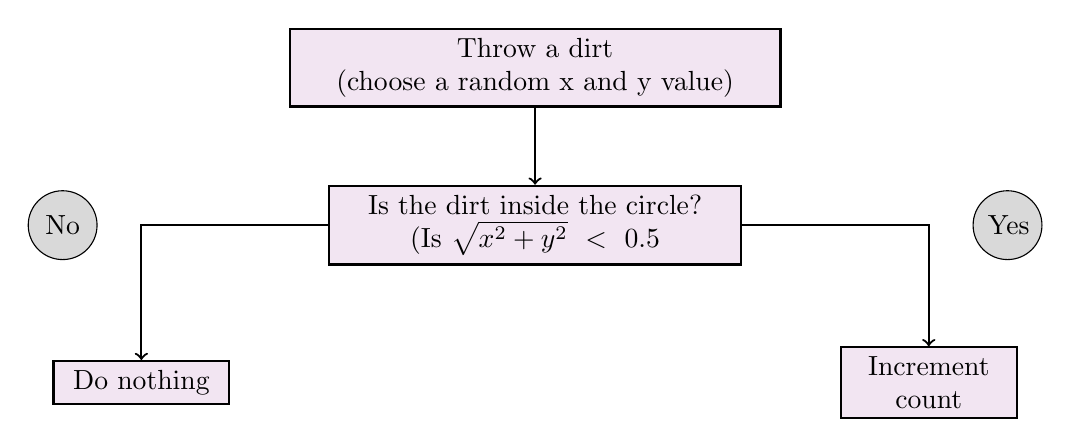
\begin{tikzpicture}
            \node[draw, rectangle, black, fill=violet!10, thick, text width=6cm, text centered] (Begin) {Throw a dirt \\(choose a random x and y value)};
            \node[draw, rectangle, black, fill=violet!10, thick, text width=5cm, text centered, below of=Begin, yshift=-1cm] (Decision) {Is the dirt inside the circle? \\(Is $\sqrt{x^2+y^2}<0.5$};
            \node[draw, rectangle, black, fill=violet!10, thick, text width=2cm, text centered, left of=Decision, xshift=-4cm, yshift=-2cm] (No) {Do nothing};
            \node[draw, rectangle, black, fill=violet!10, thick, text width=2cm, text centered, right of=Decision, xshift=4cm, yshift=-2cm] (Yes) {Increment count};
            \node[draw, circle, black, fill=gray!30, text width=0.5cm, text centered, left of=Decision, xshift=-5cm, yshift=0cm] (no) {No};
            \node[draw, circle, black, fill=gray!30, text width=0.5cm, text centered, right of=Decision, xshift=5cm, yshift=0cm] (yes) {Yes};
            \draw[black, thick, ->](Begin.south) -- (Decision.north);
            \draw[black, thick, ->](Decision.east) -| (Yes.north);
            \draw[black, thick, ->](Decision.west) -| (No.north);
            \end{tikzpicture}
        \end{center}
    \item \textbf{Estimate Pi:} If this is done for a bunch of points, the number of points inside divided by the number of total points will be the area of the circle divided by the area of the square, that is, $\frac{\pi}{4}$.
    \item \textbf{Repeat the Process:} Once we get to a couple hundred thousand, we start to get a relatively reasonable approximation for $\pi$.
     \begin{table}[h]
        \centering
        \begin{tabular}{ccc}
        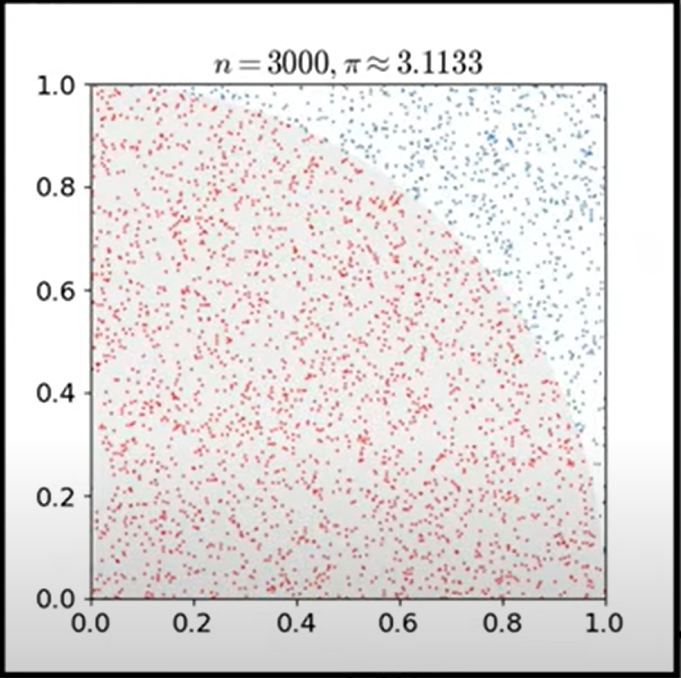
\includegraphics[scale=0.25]{figures/pi2.png}
        &         
        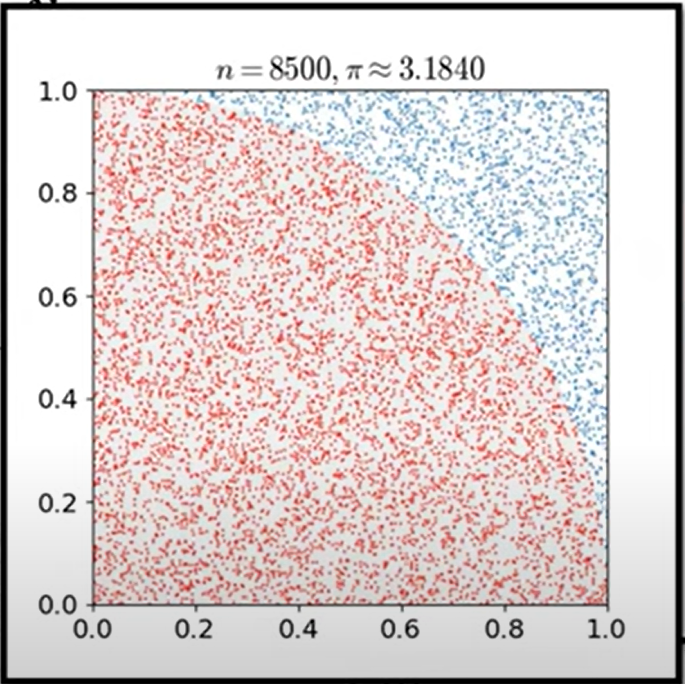
\includegraphics[scale=0.25]{figures/pi1.png} 
        &         
        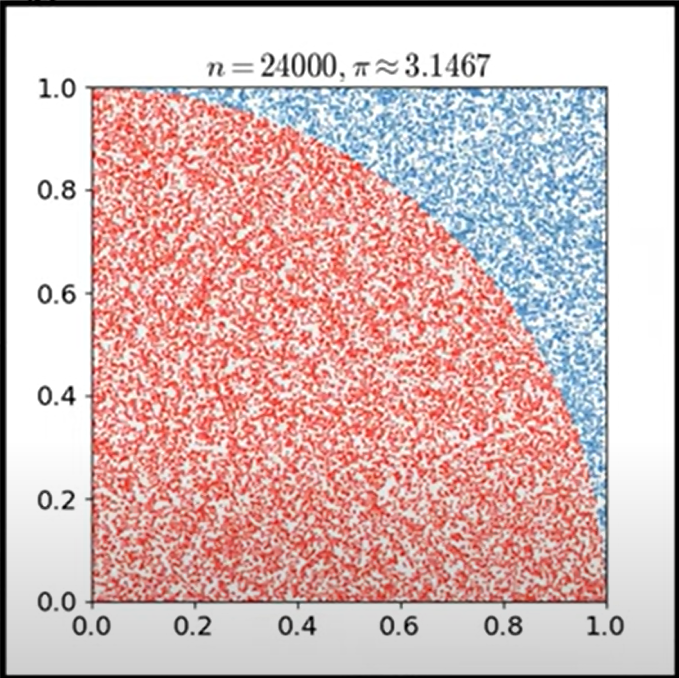
\includegraphics[scale=0.25]{figures/pi3.png}\\
        \end{tabular}
        \caption{Estimation of $\pi$}
    \end{table}
    \end{enumerate}

    \subsection{Protein Folding}
    A major difficulty in computational biology and bioinformatics is the protein folding problem, which involves estimating a protein molecule's three-dimensional shape based only on its amino acid sequence.
    \begin{figure}[h]
        \centering
        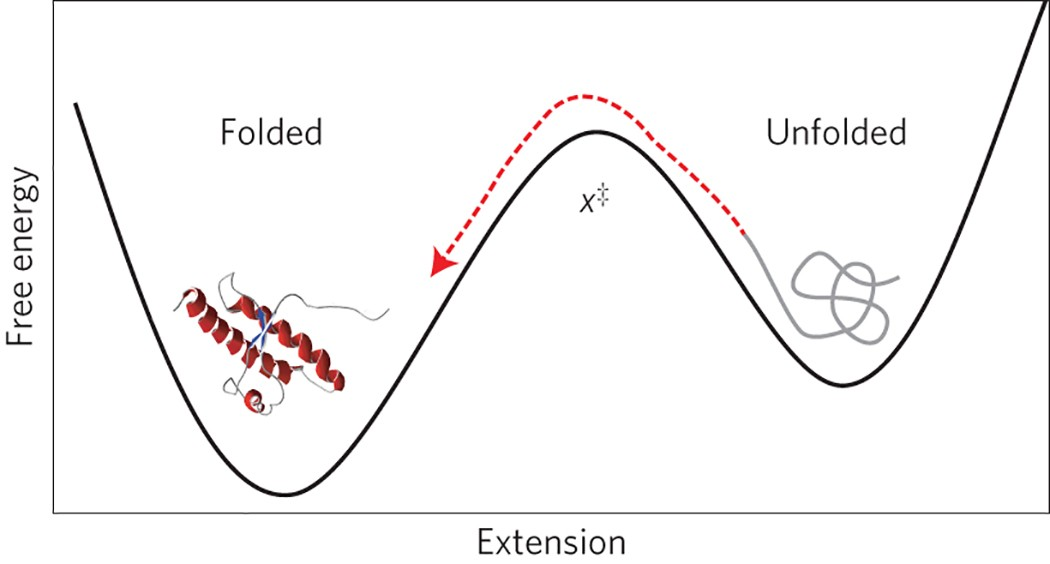
\includegraphics[width=0.8\textwidth]{figures/protein.jpeg}
        \caption{Protein folding}
    \end{figure}
    
\par Monte Carlo simulations are one method of approaching this problem's solution. Here is a thorough explanation of how to use Monte Carlo to solve the protein folding problem:
    \begin{enumerate}
        \item \textbf{Understanding Protein Folding:}
        \begin{itemize}
            \item The structure of proteins, which are made up of linear chains of amino acids, is essential to their functionality.
            \item The arrangement of amino acids makes up a protein's main structure, whilst local features like beta sheets and alpha helices are referred to as its secondary structure.
            \item The whole protein molecule is arranged in three dimensions in its tertiary structure, whereas interactions between many protein sub-units are part of the quaternary structure.
        \end{itemize}
        \item \textbf{Energy Landscape: }
        \begin{itemize}
            \item The objective of protein folding is to identify the most stable, energetically advantageous three-dimensional shape possible.
            \item Based on variables like bond lengths, angles, and non-covalent interactions (such hydrogen bonds, van der Waals forces, and hydrophobic contacts), energy functions are used to calculate how stable a protein shape is.
            \item The link between the energies associated with different protein conformations is represented by the energy landscape.
        \end{itemize}
        \item \textbf{Monte Carlo Simulation: }
        \begin{center}
            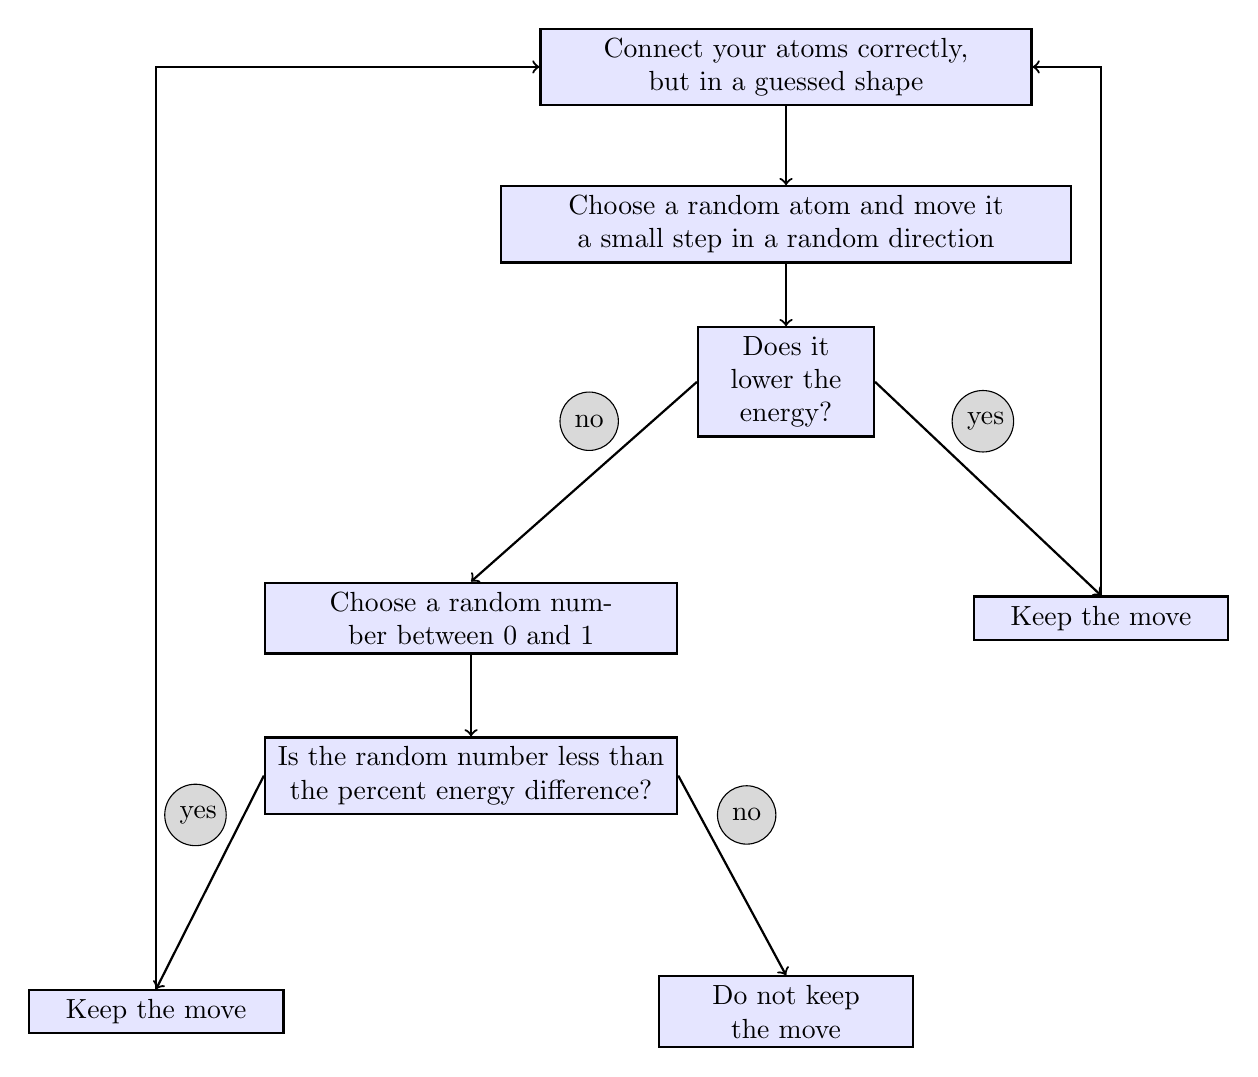
\begin{tikzpicture}
                \node[draw, rectangle, black, fill=blue!10, thick, text width=6cm, text centered] (no1) {Connect your atoms correctly,\\ but in a guessed shape};
                \node[draw, rectangle, black, fill=blue!10, thick, text width=7cm, text centered, below of=no1, yshift=-1cm] (no2) {Choose a random atom and move it a small step in a random direction};
                \node[draw, rectangle, black, fill=blue!10, thick, text width=2cm, text centered, below of=no2, yshift=-1cm] (no3) {Does it lower the energy?};
                \node[draw, circle, black, fill=gray!30, text width=0.4cm, text centered, right of=no3, xshift=1.5cm, yshift=-0.5cm] (y) {yes};
                \node[draw, circle, black, fill=gray!30, text width=0.4cm, text centered, left of=no3, xshift=-1.5cm, yshift=-0.5cm] (y) {no};
                \node[draw, rectangle, black, fill=blue!10, thick, text width=3cm, text centered, right of=no3, xshift=3cm, yshift=-3cm] (no4) {Keep the move};
                \node[draw, rectangle, black, fill=blue!10, thick, text width=5cm, text centered, left of=no3, xshift=-3cm, yshift=-3cm] (no5) {Choose a random number between 0 and 1};
                \node[draw, rectangle, black, fill=blue!10, thick, text width=5cm, text centered, below of=no5, yshift=-1cm] (no6) {Is the random number less than the percent energy difference?};
                \node[draw, rectangle, black, fill=blue!10, thick, text width=3cm, text centered, below of=no6, xshift=-4cm, yshift=-2cm] (no7) {Keep the move};
                \node[draw, rectangle, black, fill=blue!10, thick, text width=3cm, text centered, below of=no6, xshift=4cm, yshift=-2cm] (no8) {Do not keep the move};
                \node[draw, circle, black, fill=gray!30, text width=0.4cm, text centered, left of=no6, xshift=-2.5cm, yshift=-0.5cm] (y) {yes};
                \node[draw, circle, black, fill=gray!30, text width=0.4cm, text centered, right of=no6, xshift=2.5cm, yshift=-0.5cm] (y) {no};
                \draw[black, thick, ->](no1.south) -- (no2.north);
                \draw[black, thick, ->](no2.south) -- (no3.north);
                \draw[black, thick, ->](no3.east) -- (no4.north);
                \draw[black, thick, ->](no3.west) -- (no5.north);
                \draw[black, thick, ->](no4.north) |- (no1.east);
                \draw[black, thick, ->](no5.south) -- (no6.north);
                \draw[black, thick, ->](no7.north) |- (no1.west);
                \draw[black, thick, ->](no6.west) -- (no7.north);
                \draw[black, thick, ->](no6.east) -- (no8.north);
            \end{tikzpicture}   
        \end{center}
        \begin{itemize}
            \item We correctly connect the atoms in a random guessed shape. A straight line is also fine.
            \item The next step is to choose a random atom and move it a small step in a random direction.
            \item Now we go and calculate the energy. If the energy is lower than the energy that we started with, we keep the move, chose a different atom and get it to move.
            \item If the move does not lower the energy, we choose a random number between 0 and 1 and compare the number to the percent energy difference. If the random number is less than the percent energy difference, we keep it anyway and start over. Otherwise, we do not keep the move and move the atom back. We repeat the process hundreds and hundreds of times and eventually, we can end up with a correct answer.
        \end{itemize}
    \end{enumerate}
    Here we can see a Monte Carlo simulation of a polypeptide chain step by step: 
    \begin{table}[h]
        \centering
        \begin{tabular}{cc}
        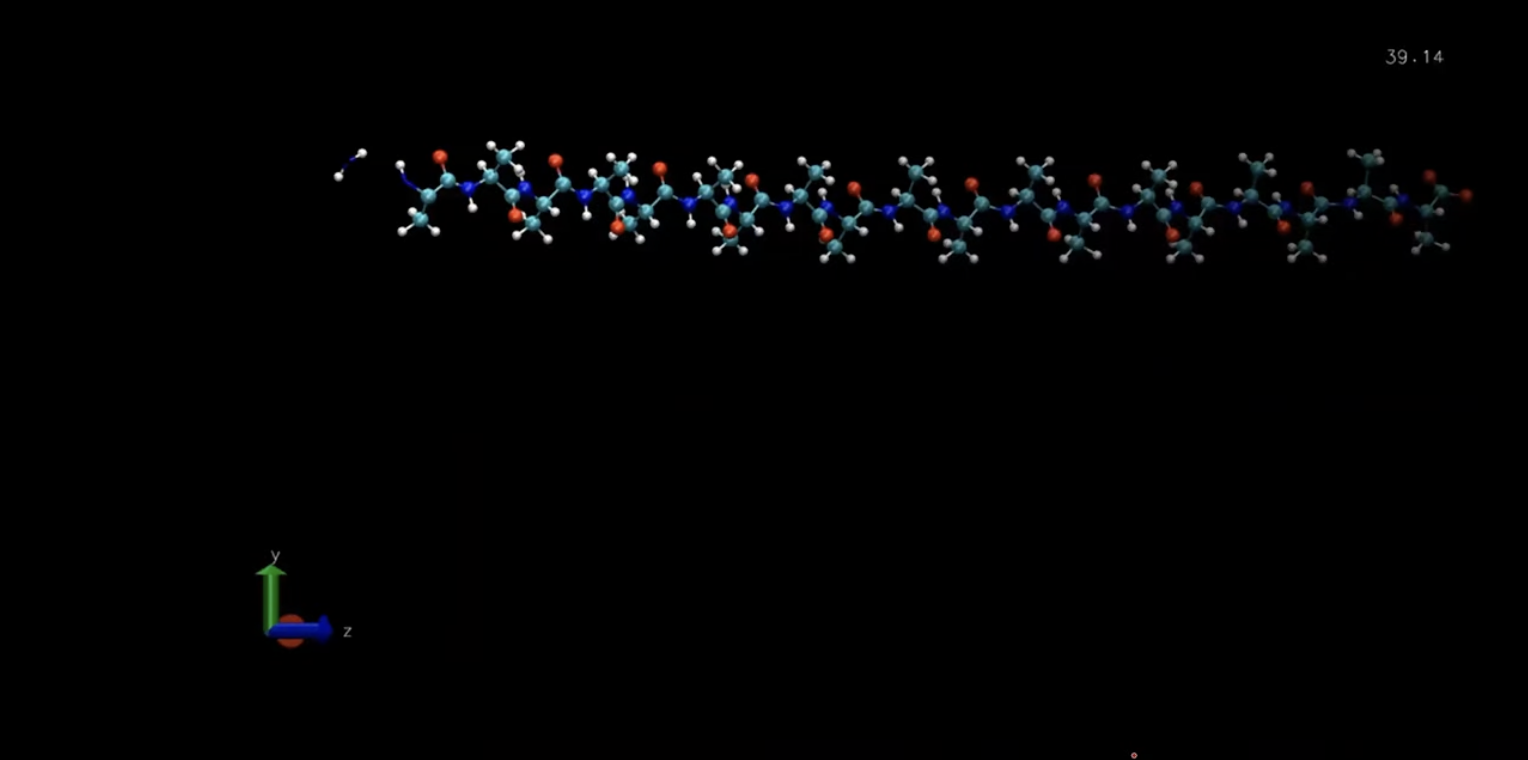
\includegraphics[width=0.45\textwidth]{figures/ap1.png}
        &         
        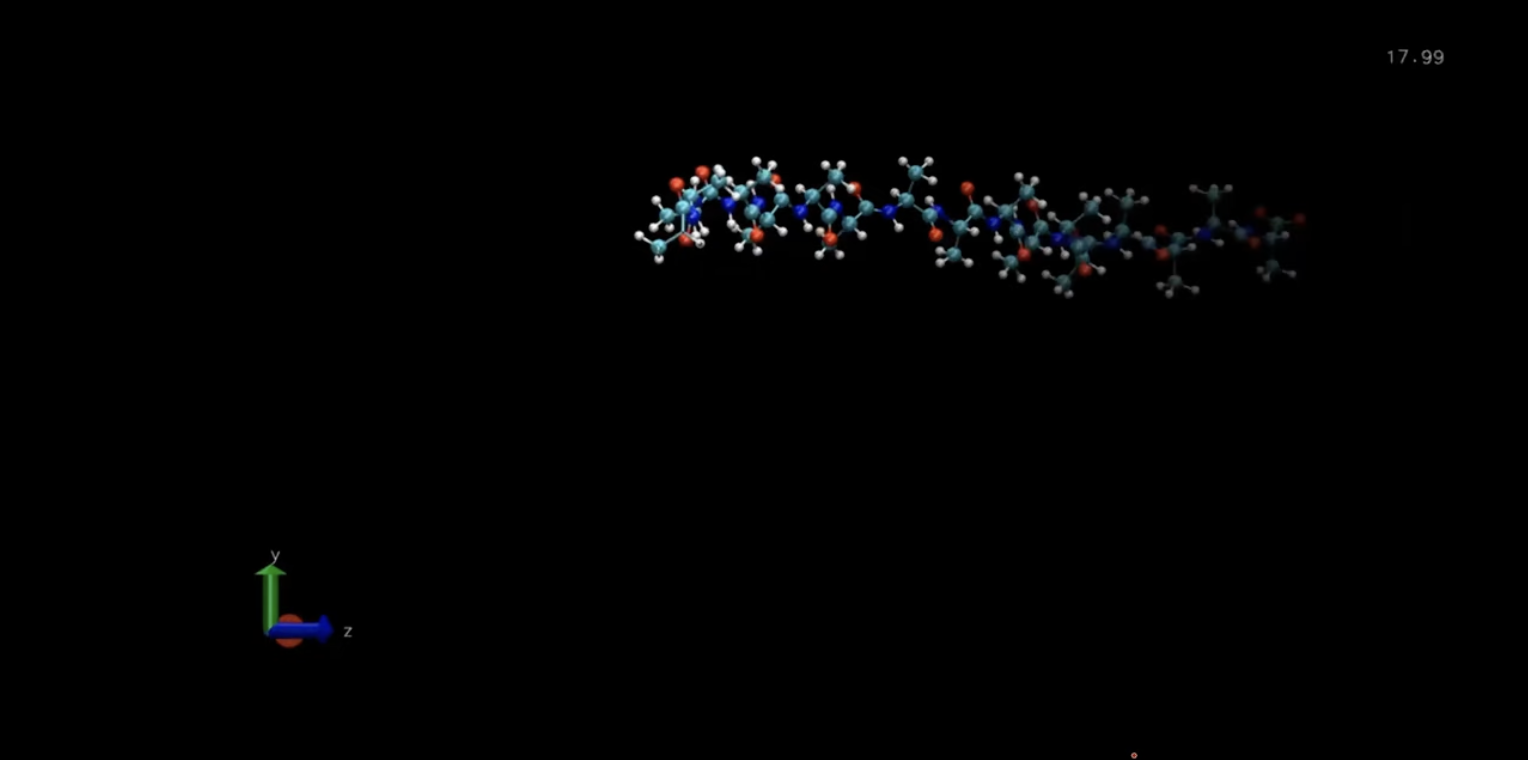
\includegraphics[width=0.45\textwidth]{figures/ap2.png} \\  
        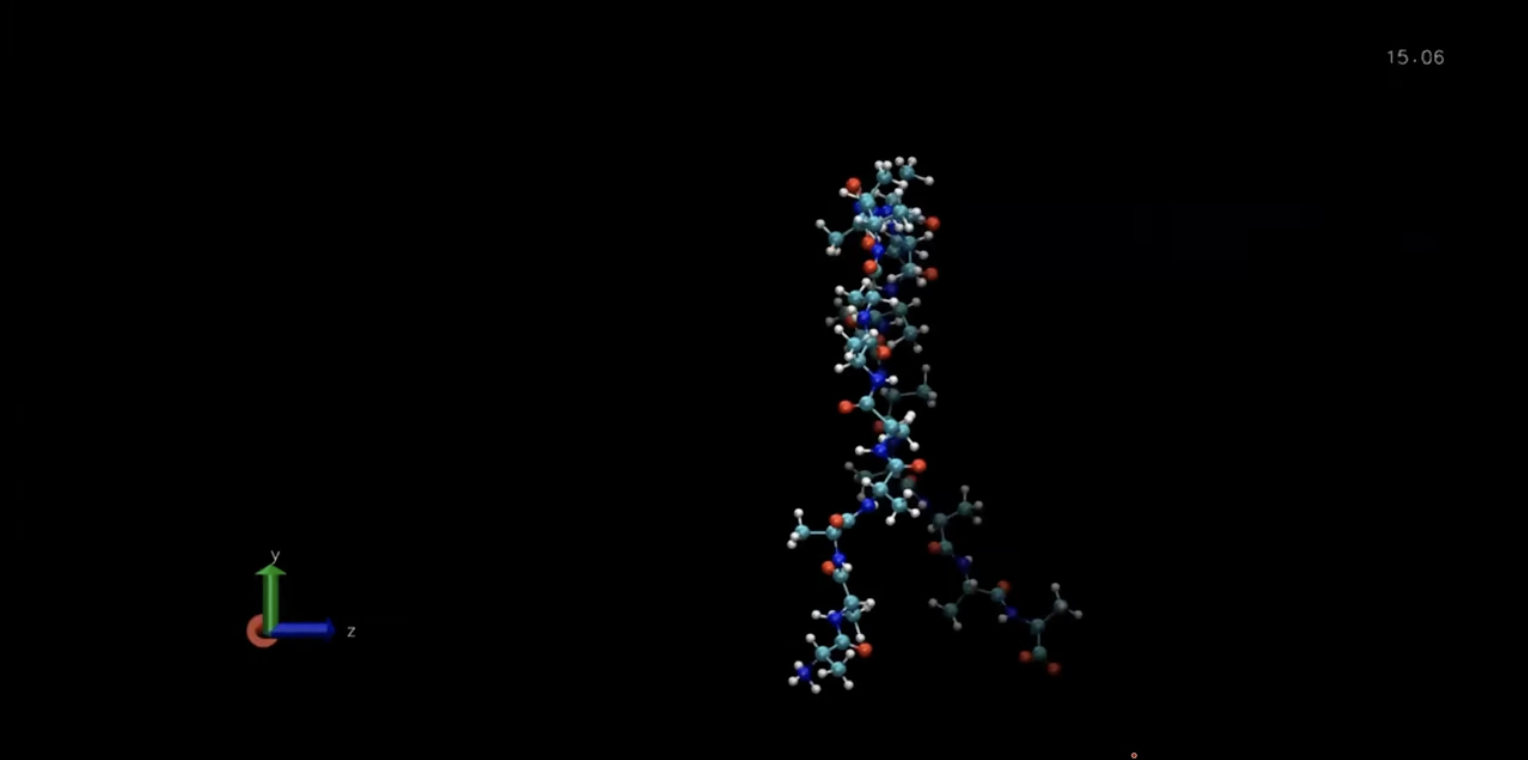
\includegraphics[width=0.45\textwidth]{figures/ap3.png}
        &         
        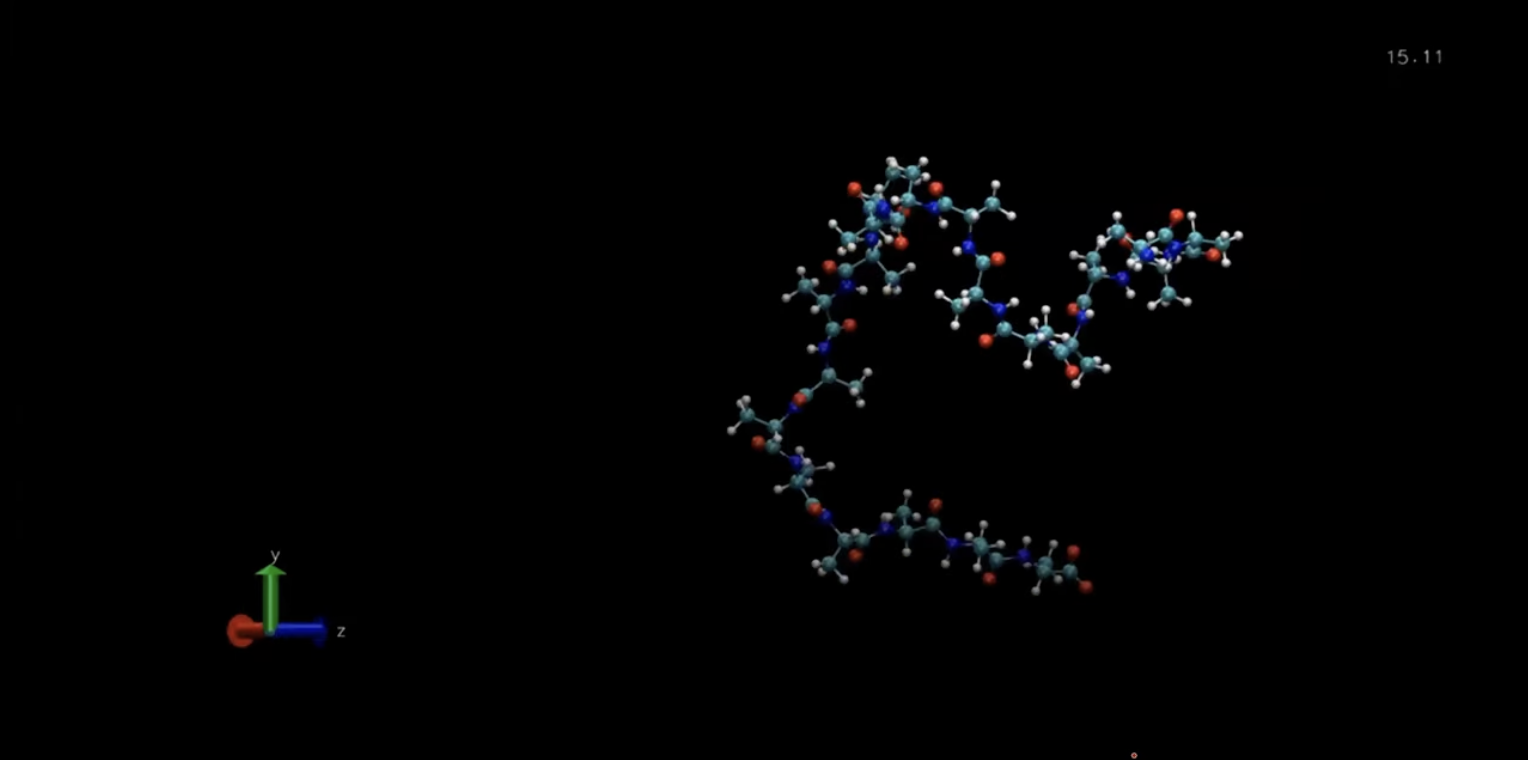
\includegraphics[width=0.45\textwidth]{figures/ap4.png}\\
        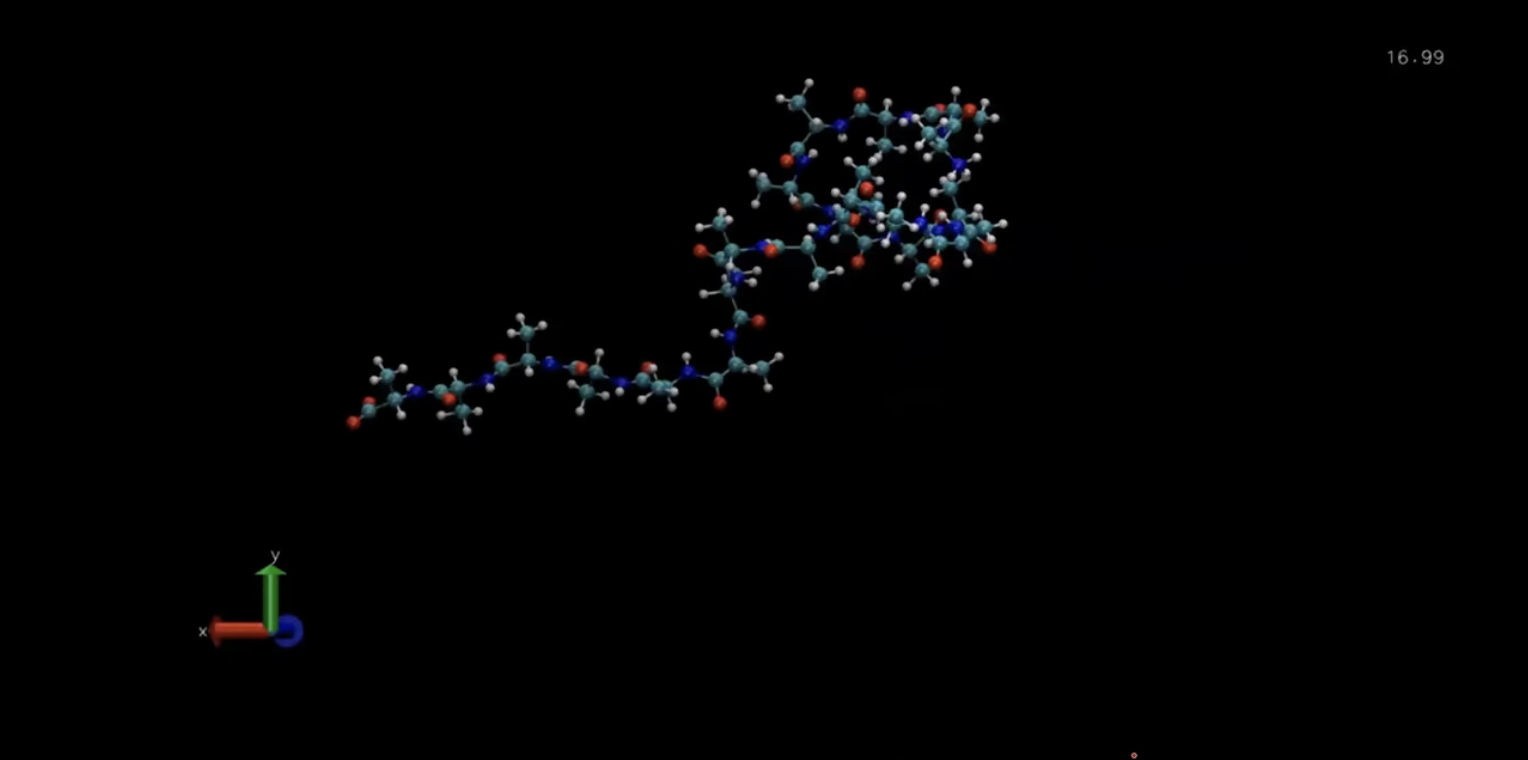
\includegraphics[width=0.45\textwidth]{figures/ap6.png}
        &         
        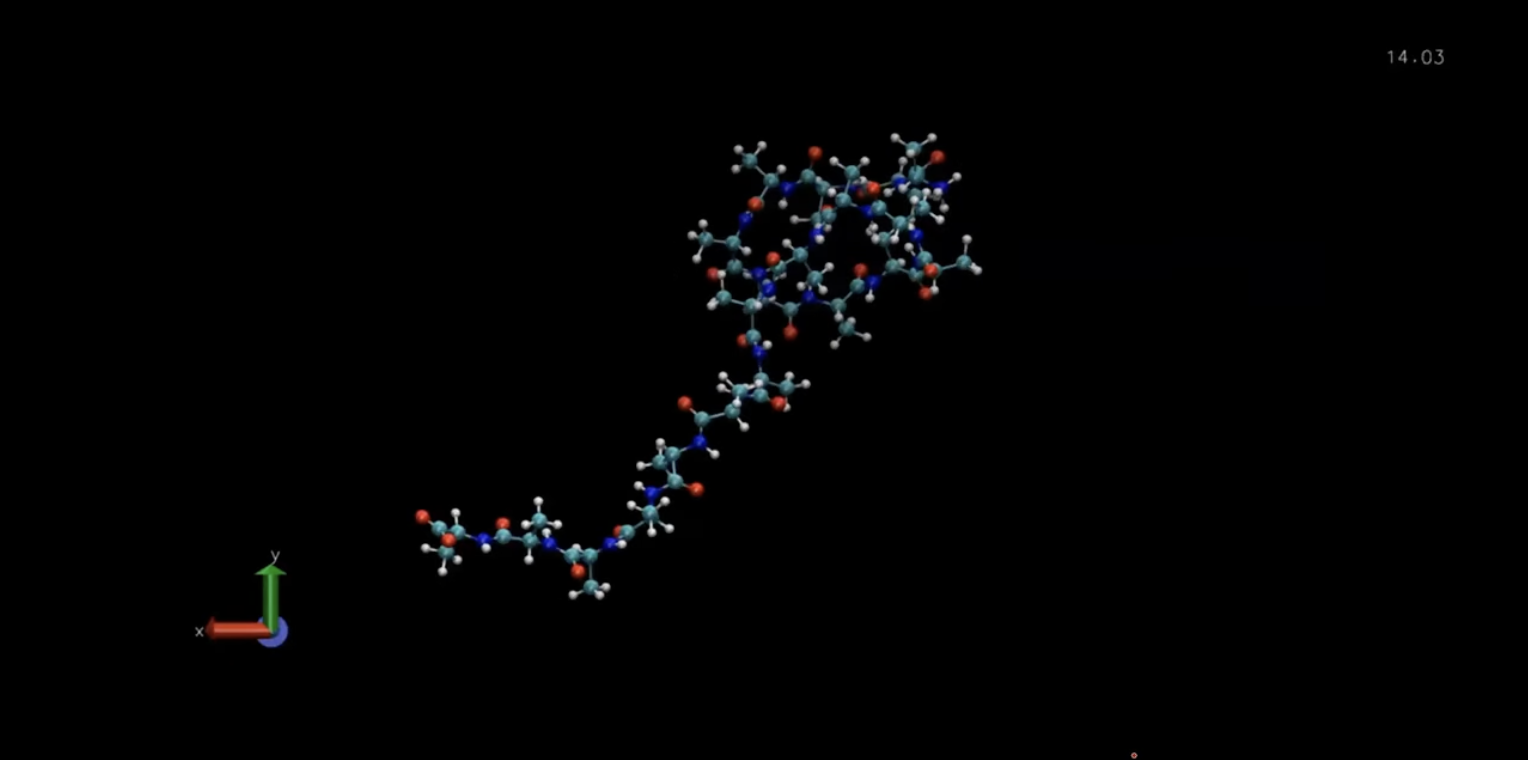
\includegraphics[width=0.45\textwidth]{figures/ap7.png}\\
        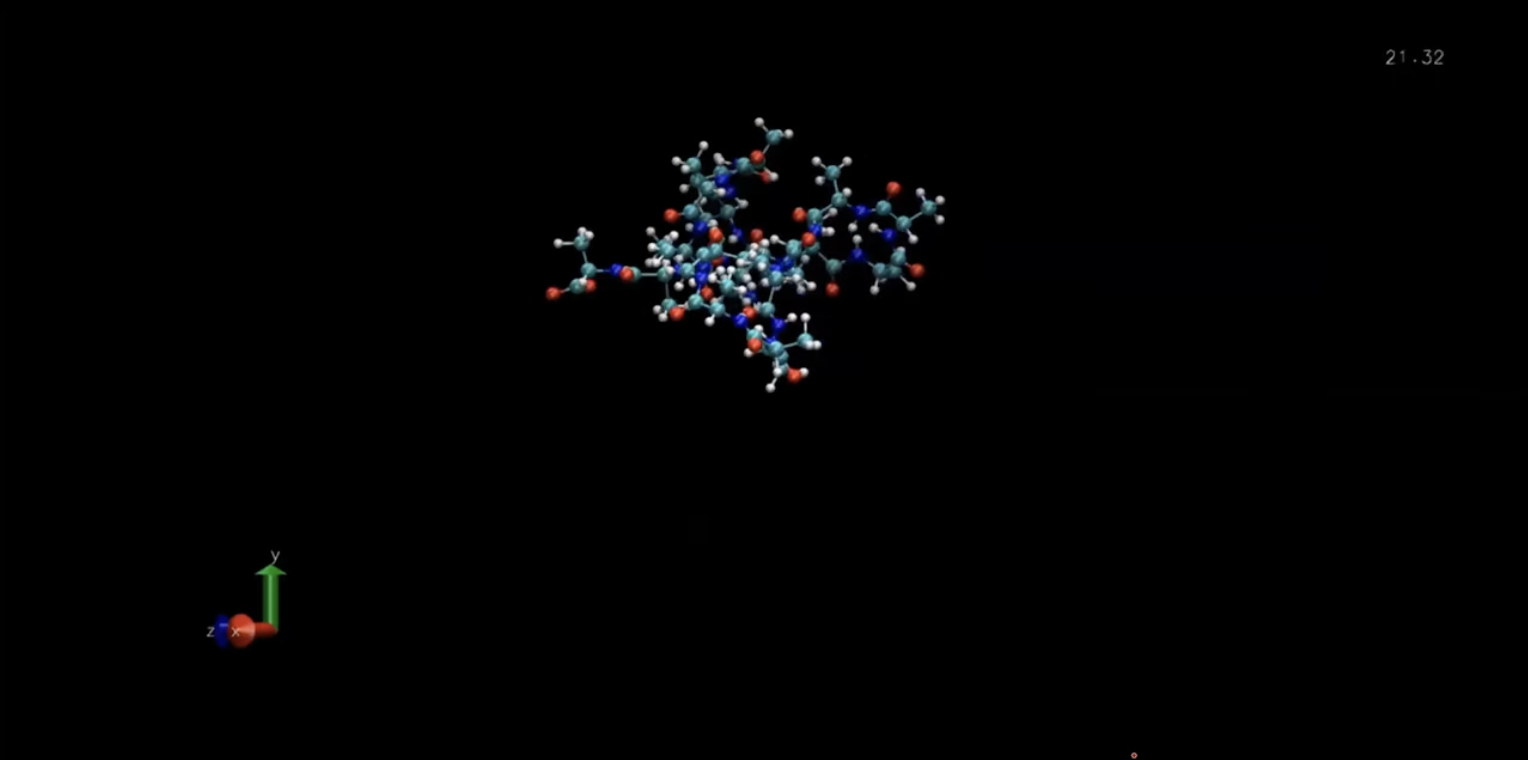
\includegraphics[width=0.45\textwidth]{figures/ap9.png}
        &         
        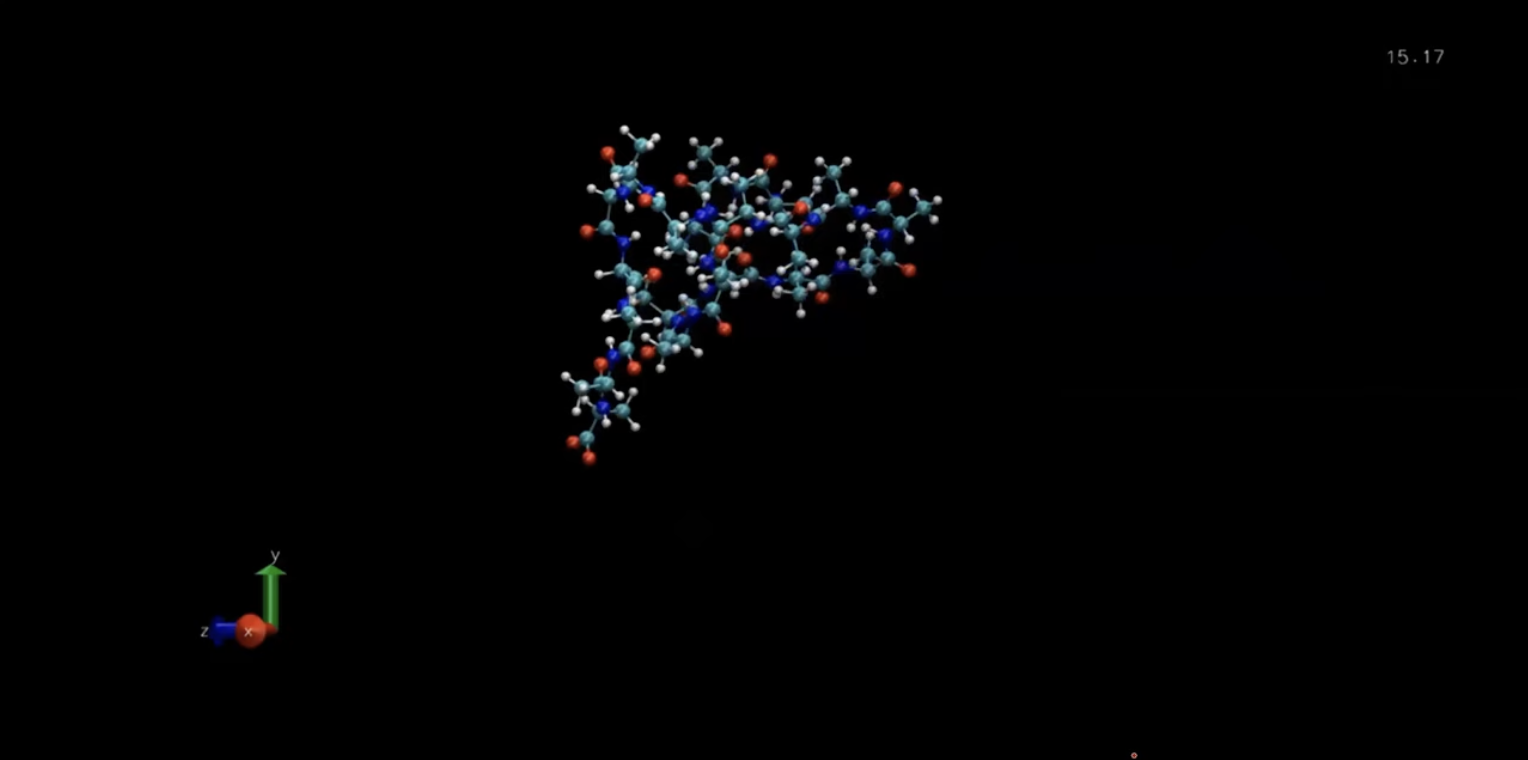
\includegraphics[width=0.45\textwidth]{figures/ap10.png}\\
        \end{tabular}
        \caption{Monte Carlo simulation of the polypeptide chain.}
    \end{table}\\
    We let the simulation run for hundreds of thousands of computations and ultimately it settles down to what the correct answer is.

    \section{Summary}
    Monte Carlo (MC) methods use random numbers to solve
    problems that cannot be solved any other way.
    It is used in various fields: Physics, Biology, Geosciences, Finance, etc.
    The versatility and efficiency of Monte Carlo algorithms make them an indispensable tool for tackling computationally challenging problems across diverse domains.
    \bibliographystyle{plain}
    \bibliography{mybib}
\end{document}
